\chapter{Economic cost optimization}
\label{cha:eco_cost_opti}

% **************************** Define Graphics Path **************************
\ifpdf
    \graphicspath{{Chapter7/Figs/Raster/}{Chapter7/Figs/PDF/}{Chapter7/Figs/}}
\else
    \graphicspath{{Chapter7/Figs/Vector/}{Chapter7/Figs/}}
\fi

% **************************** Chapter Abstract ******************************
\leftskip=1cm
\noindent
\emph{Abstract of the chapter: problem, approach, main results and conclusions.}

\leftskip=0pt\rightskip=0pt

\section{Problem statement and the state of the art}

\section{Solution strategy}

\begin{equation}
 	{C_{{\mathrm{tot}}}} = {C_0} + {C_1} \cdot R + {C_{\mathrm{f}}} \cdot {P_{\mathrm{f}}}(R)
\end{equation}

\begin{equation}
 	{c_{\mathrm{tot}}} = R + \frac{{{C_{\mathrm{f}}}}}{{{C_1}}} \cdot {P_{\mathrm{f}}}(R)
\end{equation}

\section{Results and discussion}

\subsection{Comparison}

\subsubsection{Comparing partial factor and reliability based designs}

\begin{figure}[htbp!] 
	\centering    
	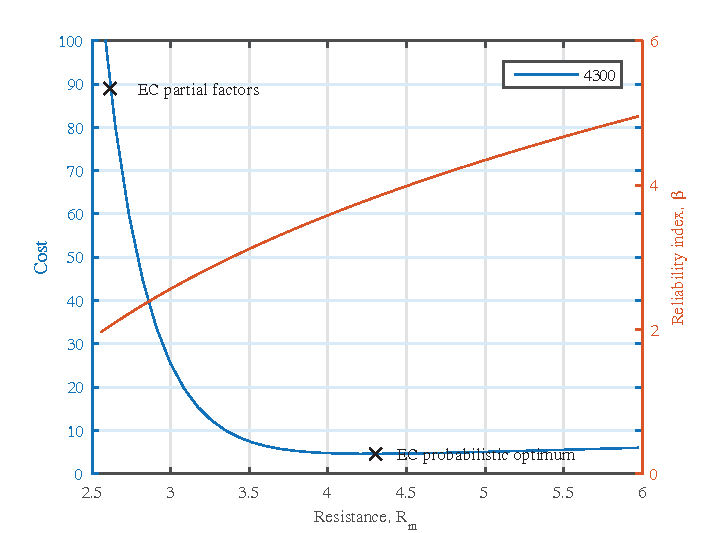
\includegraphics[width=0.7\textwidth]{cost_opti_ec_get_ratioeps_total.pdf}
	\caption{Total economic cost (blue) and reliability index (orange) as a function the mean resistance ($R_\mathrm{m}$); the designs obtained by partial factor and reliability based calculations are illustrated by a cross.}
	\label{fig:cost_opti_ec_total}
\end{figure}

\begin{figure}[htbp!] 
	\centering    
	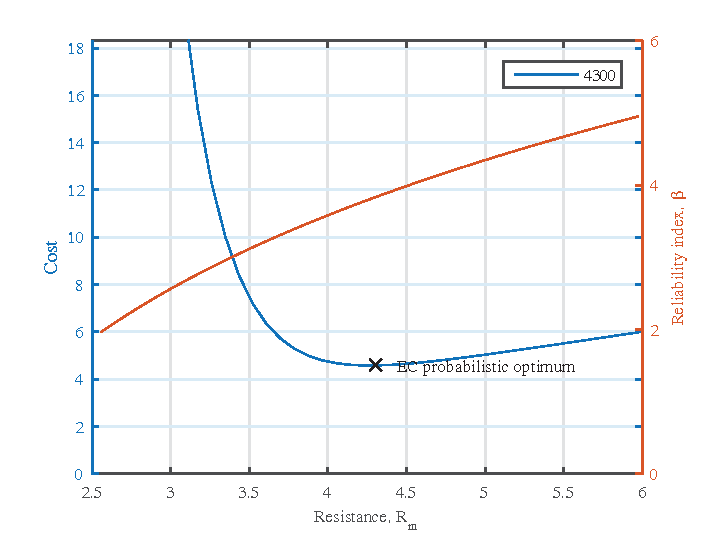
\includegraphics[width=0.7\textwidth]{cost_opti_ec_get_ratioeps_zoom.pdf}
	\caption{Same as Fig. \ref{fig:cost_opti_ec_total} but zoomed to the economic optimum.}
	\label{fig:cost_opti_ec_zoom}
\end{figure}


\subsubsection{Comparing Gumbel (EC) and BMA based optimum points}

\begin{figure}[htbp!] 
	\centering    
	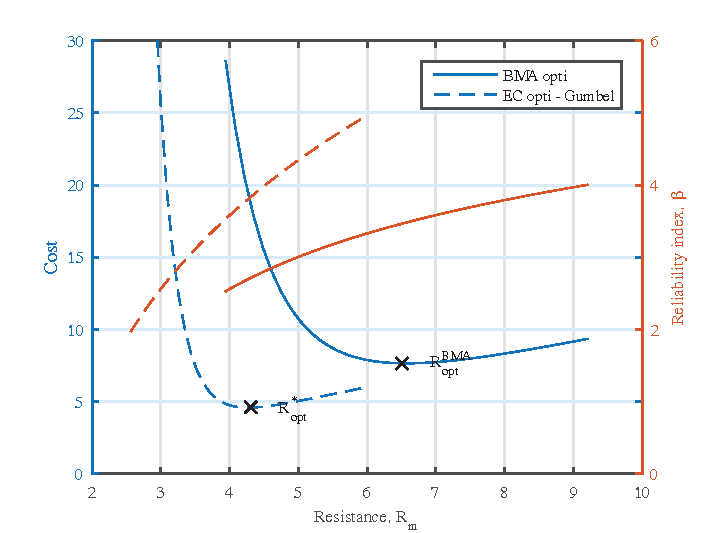
\includegraphics[width=0.7\textwidth]{cost_opti_compare_ec_bma.pdf}
	\caption{Optimum values with Gumbel and BMA models using the same ${C_{\mathrm{f}}}/{C_1}$ ratio.}
	\label{fig:cost_opti_ec_bma}
\end{figure}

Comparison of EC partial factor based design, EC cost optimization, both using Gumbel distribution and BMA cost optimization is summarized in Table \ref{tab:cost_opti_comp}.

% notes should be added
\begin{table}
\caption{Comparison of methods and models with different variable action model.}
\centering
\label{tab:cost_opti_comp}
\small
	\begin{threeparttable}
	\begin{tabular}{m{1cm} m{3cm} m{3cm} m{3cm}}
		\toprule
		  & EC partial factor, Gumbel  & EC opti, Gumbel & BMA opti \\
		\midrule
		$R_\mathrm{m}$ & 2.62 & 4.27 & 6.57  \\
		
		$\beta$ & 2.05\tnote{*} & 3.80\tnote{\textdagger} & 3.48 \\
		
		$c_\mathrm{tot}$ & 89.0 & 4.57 &  7.64 \\
		\bottomrule
	\end{tabular}
	\begin{tablenotes}
	    \item[*] assuming that $Q$ is Gumbel distributed.
	    \item[\textdagger] consequence of the initial assumption, Section ?.
	\end{tablenotes}
	\end{threeparttable}
\end{table}

\subsubsection{Reliability index for 1-year reference period}

\subsubsection{Comparing Gumbel and BMA models for different ${C_{\mathrm{f}}}/{C_1}$ ratios}

\begin{itemize}
	\item The difference between Gumbel and BMA economic optimal resistances is increasing with increasing $C_f/C_1$ ratio.
	\item RC2 and RC3 partial factors yield to design which is optimal for ${C_{\mathrm{f}}}/{C_1}$ ratio multiple order of magnitude smaller than the one calculated in Section ?? by inverse analysis.
	\item The optimal reli index varies significantly with the ${C_{\mathrm{f}}}/{C_1}$ ratio.
\end{itemize}


\begin{figure}[htbp!] 
	\centering    
	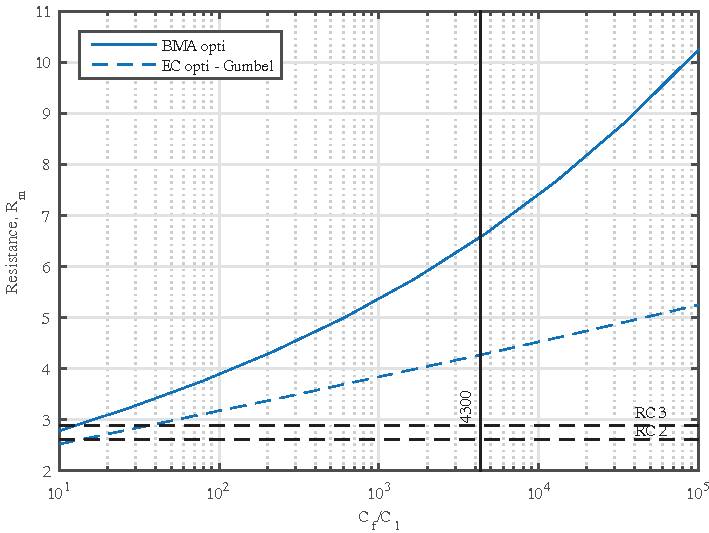
\includegraphics[width=0.7\textwidth]{comp_gumbel_bma_cf_c1_par.pdf}
	\caption{Mean resistances corresponding to economic optimum per different ${C_{\mathrm{f}}}/{C_1}$ ratios.}
	\label{fig:comp_gumbel_bma_res}
\end{figure}

\begin{figure}[htbp!] 
	\centering    
	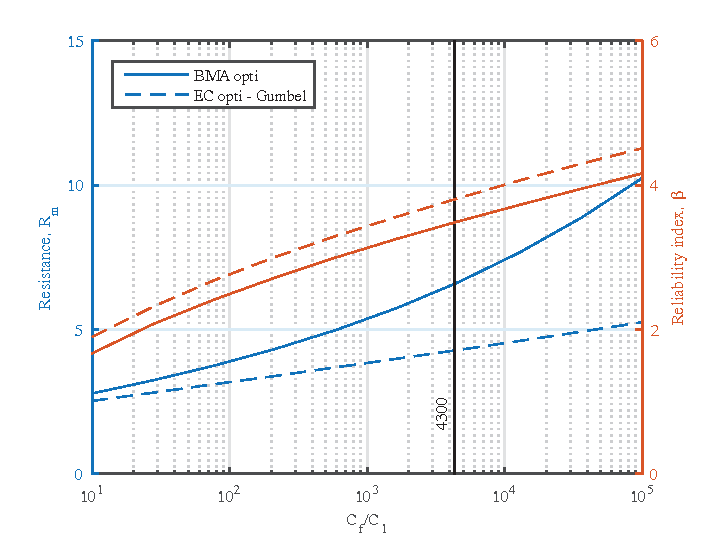
\includegraphics[width=0.7\textwidth]{comp_gumbel_bma_cf_c1_par_beta.pdf}
	\caption{Mean resistances and reliability indices corresponding to economic optimum per different ${C_{\mathrm{f}}}/{C_1}$ ratios.}
	\label{fig:comp_gumbel_bma_res_beta}
\end{figure}

\begin{figure}[htbp!] 
	\centering    
	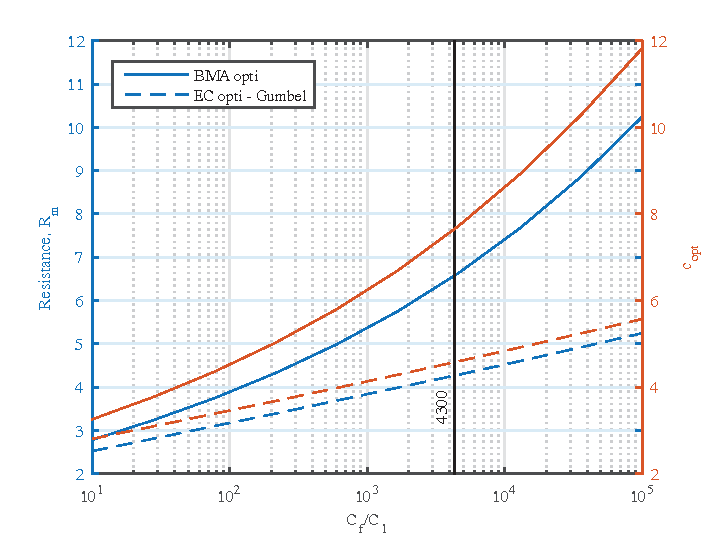
\includegraphics[width=0.7\textwidth]{comp_gumbel_bma_cf_c1_par_c_opt.pdf}
	\caption{Mean resistances and optimum costs corresponding to economic optimum per different ${C_{\mathrm{f}}}/{C_1}$ ratios.}
	\label{fig:comp_gumbel_bma_res_cost}
\end{figure}

\subsection{Partial factor for snow action}

Comments could be made on how the partial factor would change by incorporating parameter estimation uncertainty and by switching from Gumbel to GEV or other distribution types.
This a delicate question since it is well known that the current Eurocode recommendations do not provide the target reliability stipulated in \citep{EN0}. It is hard to separate the effects, though I believe it would convey interesting information.
Maybe Chapter \ref{cha:stat_unc} suits better for this analysis.

%\section{Extension to other random variables}

\section{Application example}

\section{Summary and conclusions}

